\documentclass[a4paper,12pt]{report}

\usepackage[utf8x]{inputenc}
\usepackage[T2A]{fontenc}
\usepackage[english, russian]{babel}

% Опционно, требует  apt-get install scalable-cyrfonts.*
% и удаления одной строчки в cyrtimes.sty
% Сточку не удалять!
% \usepackage{cyrtimes}

% Картнки и tikz
\usepackage{graphicx}
\usepackage{tikz}
\usetikzlibrary{snakes,arrows,shapes}


% Увы, поля придётся уменьшить из-за листингов.
\topmargin -1cm
\oddsidemargin -0.5cm
\evensidemargin -0.5cm
\textwidth 17cm
\textheight 24cm

\sloppy



% Оглавление в PDF
\usepackage[
bookmarks=true,
colorlinks=true, linkcolor=black, anchorcolor=black, citecolor=black, menucolor=black,filecolor=black, urlcolor=black,
unicode=true
]{hyperref}

% Для исходного кода в тексте
% \newcommand{\Code}[1]{\texttt{#1}}

% Некоторая русификация.
% \usepackage{misccorr} % Oh shi^W^W, оно не работает с report.
\usepackage{indentfirst}
\renewcommand{\labelitemi}{\normalfont\bfseries{--}}

% На дворе XXI век, но пакет listings всё ещё не пашет с русскими комментариями!

% Пакет listings для простой вставки исходников
% \usepackage{listings}
% Параметры оформления
% \lstset{
% showspaces=false,
% showtabs=false,
% frame=single,
% tabsize=4,
% basicstyle=\ttfamily,
% identifierstyle=\ttfamily,
% commentstyle=\itshape,
% stringstyle=\ttfamily,
% keywordstyle=\ttfamily,
% breaklines=true
% }
% Русский в комментариях.
% \lstset{escapebegin=\begin{cyr},escapeend=\end{cyr}}



% А это взято из файла, сгенерённого doxygen
\usepackage{calc}
\usepackage{array}
\newenvironment{Code}
{\footnotesize}
{\normalsize}
\newcommand{\doxyref}[3]{\textbf{#1} (\textnormal{#2}\,\pageref{#3})}
\newenvironment{DocInclude}
{\footnotesize}
{\normalsize}
\newenvironment{VerbInclude}
{\footnotesize}
{\normalsize}
\newenvironment{Image}
{\begin{figure}[H]}
{\end{figure}}
\newenvironment{ImageNoCaption}{}{}
\newenvironment{CompactList}
{\begin{list}{}{
  \setlength{\leftmargin}{0.5cm}
  \setlength{\itemsep}{0pt}
  \setlength{\parsep}{0pt}
  \setlength{\topsep}{0pt}
  \renewcommand{\makelabel}{\hfill}}}
{\end{list}}
\newenvironment{CompactItemize}
{
  \begin{itemize}
  \setlength{\itemsep}{-3pt}
  \setlength{\parsep}{0pt}
  \setlength{\topsep}{0pt}
  \setlength{\partopsep}{0pt}
}
{\end{itemize}}
\newcommand{\PBS}[1]{\let\temp=\\#1\let\\=\temp}
\newlength{\tmplength}
\newenvironment{TabularC}[1]
{
\setlength{\tmplength}
     {\linewidth/(#1)-\tabcolsep*2-\arrayrulewidth*(#1+1)/(#1)}
      \par\begin{tabular*}{\linewidth}
             {*{#1}{|>{\PBS\raggedright\hspace{0pt}}p{\the\tmplength}}|}
}
{\end{tabular*}\par}
\newcommand{\entrylabel}[1]{
   {\parbox[b]{\labelwidth-4pt}{\makebox[0pt][l]{\textbf{#1}}\vspace{1.5\baselineskip}}}}
\newenvironment{Desc}
{\begin{list}{}
  {
    \settowidth{\labelwidth}{40pt}
    \setlength{\leftmargin}{\labelwidth}
    \setlength{\parsep}{0pt}
    \setlength{\itemsep}{-4pt}
    \renewcommand{\makelabel}{\entrylabel}
  }
}
{\end{list}}
\newenvironment{Indent}
  {\begin{list}{}{\setlength{\leftmargin}{0.5cm}}
      \item[]\ignorespaces}
  {\unskip\end{list}}



\title{Отчёт по курсовому проекту}
\author{(Бородин Дмитрий Сергеевич, Федоров Павел Вячеславович)}

\begin{document}

\maketitle

\tableofcontents

\addcontentsline{toc}{chapter}{Введение}
\chapter*{Введение}

\section*{Сервер}

\subsection{Задание. 6}
Используется вызов select и рабочие процессы. Журналирование в отдельном процессе.
\subsection{Цели и задачи}
Цель: 
    Разработать \textbf{SMTP-сервер} с использованием рабочих процессов и select.

Задачи:
\begin{itemize}
    \item Проанализировать архитектурное решение
    \item Разработать подход для обработки входящих соединений и хранения входящих писем в maildir
    \item Рассмотреть \textbf{SMTP}-протокол
    \item Реализовать программу для получения писем по протоколу \textbf{SMTP}
\end{itemize}

\section{Клиент}

\subsection{Задание. 26}
Используется вызов pselect и рабочие потоки. Журналирование в отдельном потоки. Не обязательно пытаться отправлять все сообщения для одного MX за одну сессию.
\subsection{Цели и задачи}
Цель: 
    Разработать \textbf{SMTP-клиент} с использованием рабочих потоков и pselect.

Задачи:
\begin{itemize}
    \item Проанализировать архитектурное решение maildir
    \item Разработать подход для обработки писем в maildir 
    \item Рассмотреть \textbf{SMTP}-протокол
    \item Проанализировать способы получения и обработки \textbf{MX}-записей
    \item Реализовать программу для отправки писем по протоколу \textbf{SMTP}
\end{itemize}


% Два предложения о содержании отчёта. Для нового абзаца в исходном тексте должна быть пустая строка.

% Это~-- шаблон отчёта (вот как оформляется длинное тире, перед котрым идёт неразрывный пробел).


% Здесь должно быть вербальное задание.

% А вот так оформляются списки:
% \begin{itemize}
% \item элемент списка;
% \item последний элемент списка.
% \end{itemize}

% Нумерованный список выглядит следующим образом.
% \begin{enumerate}
% \item Первый элемент.
% \item Второй элемент.
% \end{enumerate}

\chapter{Аналитический раздел}
\section{Предметная область}
\subsection{ER-диаграмма предметной области}
Согласно обозначенному протоколу в рамках данной работы, в системе устанавливаются отношения "отправитель - получатель", причем отправитель может отправить несколько писем, указав себя в качестве источника сообщения (единственного). Основная единица данных, передаваемая по протоколу - письмо, которое включает в себя отправителя и получателя, причем получателей может быть несколько. Также письмо содержит в себе единственное тело, которое может быть использовано как для последующей передачи, так и для хранения на сервере.
Таким образом, в рамках предметной области можно выделить 4 вида сущностей:
\begin{itemize}
    \item 1. Отправитель
    \item 2. Получатель
    \item 3. Письмо
    \item 4. Тело письма
\end{itemize}
Зависимость между сущностями предметной области может быть описана следующей диаграммой (~\ref{fig:er_diagram} ):
\begin{figure}
\centering
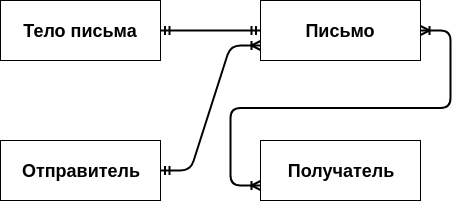
\includegraphics[width=\textwidth]{static/ER_diagram_field.png}
\caption{ER-диаграмма сущностей}
\label{fig:er_diagram}
\end{figure}

\section{Сервер}
\subsection{Преимущества и недостатки условия задачи}
Согласно условию задачи, в работе сервера предлагается исполльзовать многопроцессную систему. Данный тип системы
является самым простым в плане разработки при условии, что на каждую пользовательскую сессию или даже любой пользовательский запрос
создается новый процесс. Данная архитектура имеет следующие преимущества:
\begin{itemize}
    \item 1. Простота разработки. Фактически, мы запускаем много копий однопоточного приложения и они работают независимо друг от друга. Можно не использовать никаких специфически многопоточных API и средств межпроцессного взаимодействия.
    \item 2. Высокая надежность. Аварийное завершение любого из процессов никак не затрагивает остальные процессы.
    \item 3. Хорошая переносимость. Приложение будет работать налюбой многозадачной ОС
    \item 4. Высокая безопасность. Разные процессы приложения могут запускаться от имени разных пользователей. Таким образом можно реализовать принцип минимальных привилегий, когда каждый из процессов имеет лишь те права, которые необходимы ему для работы. Даже если в каком-то из процессов будет обнаружена ошибка, допускающая удаленное исполнение кода, взломщик сможет получить лишь уровень доступа, с которым исполнялся этот процесс.
\end{itemize}
При этом данная архитектура имеет следующие недостатки:
\begin{itemize}
    \item 1. Далеко не все прикладные задачи можно предоставлять таким образом. Например, эта архитектура годится для сервера, занимающегося раздачей статических HTMLстраниц, но совсем непригодна для сервера баз данных и многих серверов приложений.
    \item 2. Создание и уничтожение процессов – дорогая операция, поэтому для многих задач такая архитектура неоптимальна.
\end{itemize}
Поэтому для минимизации операций создания и уничтожения процессов предлагается архитектурное решение, представляющее собой пул процессов,
создаанных заранее. Это позволит фиксировать число операций создания процесса. При этом слушающие сокеты сервера должны наследоваться каждым создаваемым процессом. Это делается для решения проблемы распределения соединений между процессами одной группы. В ходе исследования предметной области и реализации сервера с заданной архитектурой, было выяснено, что открытые файловые дескрипторы процесса не могут быть переданы посредством очередей сообщений. (при передаче открытого дескриптора возникает ошибка EBADF). Однако система с наследованием имеет недостаток в отсутствии возможности распределения соединений между процессами - соединение принимает тот, кто быстрее успел.

% \section{Клиент}

% \subsection{Алгоритм}

\chapter{Конструкторский раздел}

\section{Сервер}

\subsection{Конечный автомат состояний сервера}

Рис.~\ref{fig:server_fsm} нагенерил самодельный \textit{fsm2dot} из \textit{autogen} и \textit{dot2tex} на пару \textit{dot}. Никто не мешает изменить параметры типа \textit{rankdir} прямо в \textit{fsm2dot}, если он будет лучше смотреться, например, сверху-вниз.

\begin{figure}
\centering
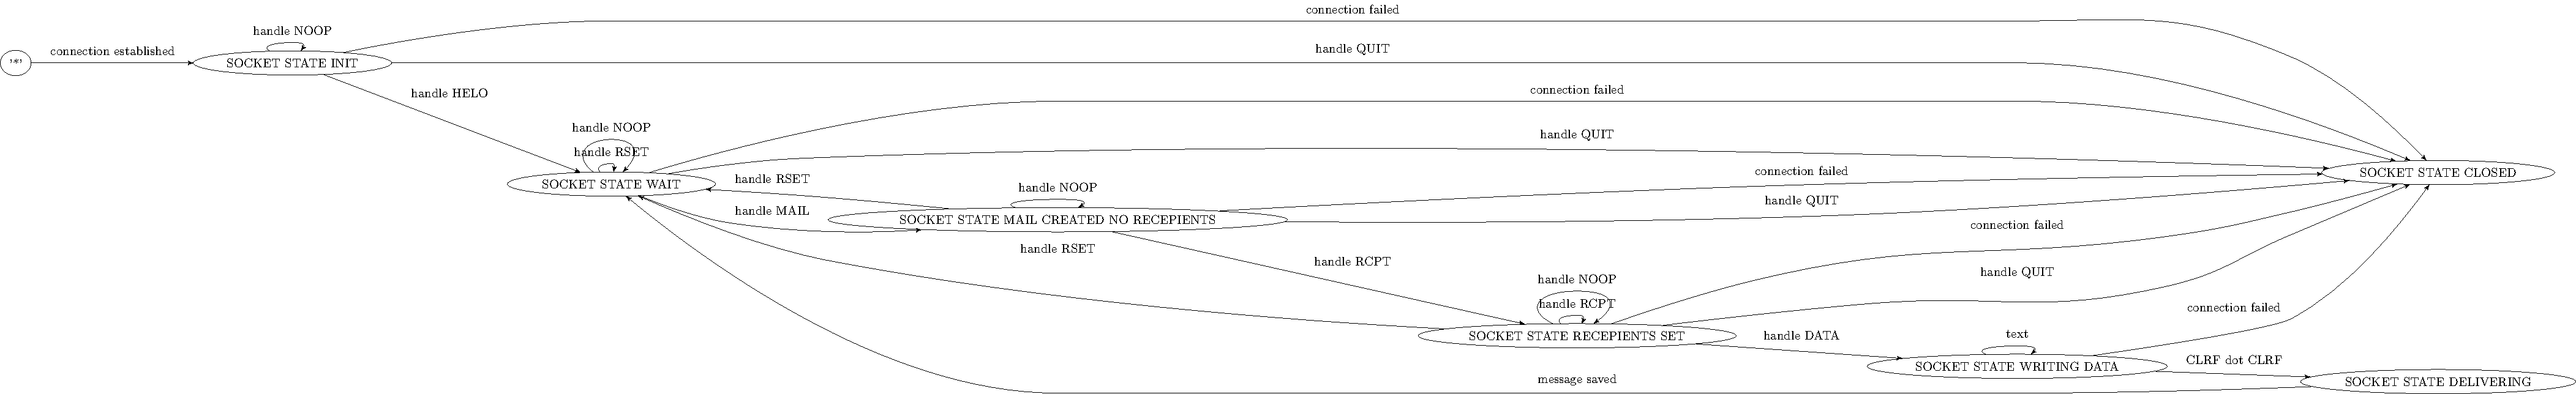
\includegraphics[width=\textwidth]{static/server_dot.pdf}
\caption{Состояния сервера}
\label{fig:server_fsm}
\end{figure}

\subsection{Синтаксис команд протокола}
Ниже приведен формат команд сообщений протокола в виде регулярных выражений
\begin{enumerate}
\item \textbf{EHLO}: {\it EHLO [w+]+\/}
\item \textbf{HELO}: {\it HЕLO [w+]+\/}
\item \textbf{MAIL}: {\it MAIL FROM <[\textbackslash w]+@[\textbackslash w]+\.[\textbackslash w]+>\/}
\item \textbf{RCPT}: {\it RCPT <[\textbackslash w]+@[\textbackslash w]+\.[\textbackslash w]+>\/}
\item \textbf{DATA}: {\it DATA\/}
\item \textbf{NOOP}: {\it NOOP\/}
\item \textbf{RSET}: {\it RSET\/}
\item \textbf{QUIT}: {\it QUIT\/}
\end{enumerate}

\subsection{Представление данных}
Ниже приведены диаграммы представления данных в системе - логическая и физическая.

\begin{figure}
\centering
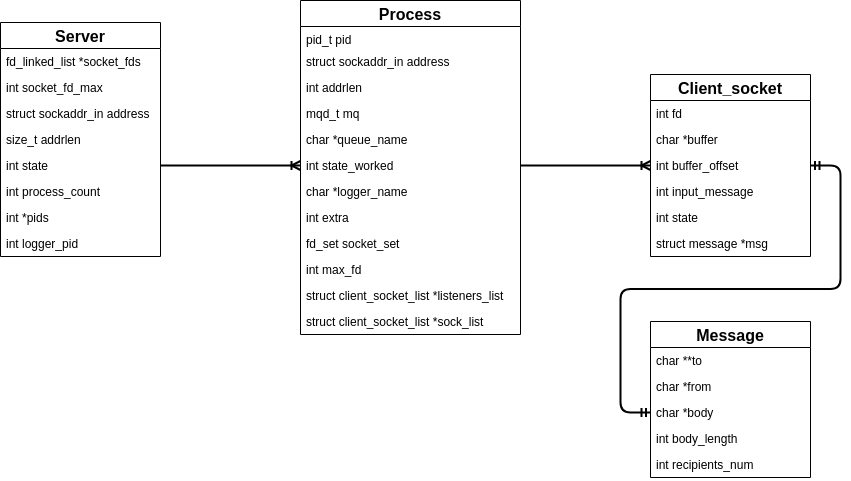
\includegraphics[width=\textwidth]{static/Server_Class_Diagram.png}
\caption{Логическая диаграмма сущностей}
\label{fig:logic_diagram}
\end{figure}

\begin{figure}
\centering
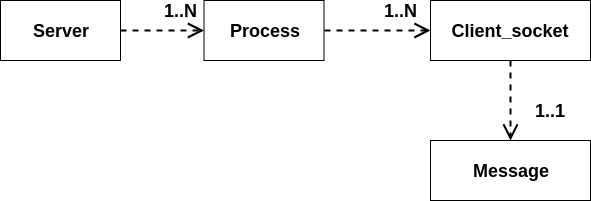
\includegraphics[width=\textwidth]{static/Physical_data.png}
\caption{Физическая диаграмма сущностей}
\label{fig:phys_diagram}
\end{figure}


\subsection{Особенности реализации}
\begin{itemize}
    \item 1. Так как, согласно предложенному варианту задания на разработкаъу сервера, предлагается реализовать многопроцессную систему с журналированием в отдельном процессе, то имеет смысл объединить сущности логгера и обычного процесса с обязательной пометкой о том, что данный процесс - процесс журналирования;
    \item 2. Создание слушающих сокетов осуществляется через метод getaddrinfo() (стандарт gnu99). Этот метод позволяет получить все сокеты на конкретном адресе (в общем случае метод для локального хоста предоставляет одну структуру, описывающую сокет для адресов IPv4, одну - для адресов IPv6)
    \item 3. Обработка таймаутов для сокетов осуществляется через пометку всех клиентских сокетов, как закрытых. Это делается для освобождения ресурсов в ожидании новых соединений. Процессы при этом не закрываются, так как согласно выбранной архитектуре число процессов фиксированно - это сделано для минимизации числа вызовов fork(). Слушающие сокеты при этом также остаются открытыми, так как их число также ограничено.
    \item 4. Graceful closing  осуществляется при помощи разделяемой памяти (очереди сообщений) и сигналов. В общем случае реализуются обработчики сигнала SIGINT для master-процесса и дочерних процессов. Для master-процесса реализуется ожидание закрытия всех дочерних процессов, после которого происходит освобождение системных ресурсов и удаление процесса, тогда как для дочерних процессов освобождение ресурсов осуществляется после получения сигнала SIGINT. Для родительского и дочерних процессов реализован схожий переход к освобождению ресурсов - через внутреннюю переменную, которая зануляется по сигналу.
    \item 5. В системе реализовано создание слушающих сокетов по числу сокетов (но в текущей версии приложения не используется, так как имеющихся сокетов при создании с помощью getaddrinfo() достаточно для функционального тестирования)
    \item 6. sleep() в родительском процессе обоснован тем, что в процессе разработки функциональность родительского процесса деградировала (см. Аналитическая часть), и для отсутствия захламеления журнала, родительский процесс с периодичностью сообщает, что жив. В случае расширения функциональности sleep() может быть убран.
    \item 7. В системе не реализовано использование конфигураций - зона ближайшего развития проекта.
    \item 8. Тестирование протокола осуществляется через мок-объекты с нулевым файловым дескриптором. Объект используется для непосредственного тестирования протокола, это позволяет гарантированно не зависать на моментах приема-передачи. Покрытие тестами неполное, так как это выходит за рамки проекта - вторая зона ближайшего развития проекта.
    \item 9. Генерация имен файлов сообщений осуществляется через структуру timeval - гарантирует относительно случайное имя.
    \item 10. Для родительского процесса аналогичным образом реализована система состояний. Но так как диаграмма состояний этого процесса малоинформативна из-за деградации функциональности, принято решение не включать ее в отчет.
    \item 11. Команда VRFY  не обрабатывается, как отдельная команда - она обрабтывается так, если бы это был любой другой текст, используемый в качестве команды.
    \item 12. Команды должны посылаться на сервер строго как 4 символа в верхнем регистре - нет перевода между регистрами
\end{itemize}

\subsection{Алгоритм обработки соединений в одном процессе}
\begin{verbatim}

\> ПОКА (процесс_работает == 1) \\
\> \> Удалить из списка клиентских сокетов процесса сокеты с состоянием "SOCKET_STATE_CLOSED" \\
\> \> Обнулить сет читателей \\
\> \> Добавить дескрипторы слушающих сокетов в сет читателей \\
\> \> Добавить дескрипторы клиентских сокетов в сет читателей \\
\> \> Добавить дескриптор очереди сообщений в сет читателей \\ 
\> \> Ожидать соединения на одном из сокетов (время = 15с) \\
\> \> ЕСЛИ (количество_свободных_сокетов == 0) ТО \\
\> \> \> Обработать таймаут, переведя все клиентские сокеты в состояние "SOCKET_STATE_CLOSED" \\
\> \> ИНАЧЕ \\
\> \> \> ЕСЛИ действие на очереди сообщений ТО \\
\> \> \> \> Проверить запрос на graceful shutdown \\
\> \> \> \> ЕСЛИ есть запрос ТО \\
\> \> \> \> \> процесс_работает = 0 \\
\> \> \> ДЛЯ каждого слушающего сокета \\
\> \> \> \> ЕСЛИ действие на одном из слушающих сокетов ТО \\
\> \> \> \> \> Принять новое соединение \\
\> \> \> \> \> Инициализировать новый сокет \\
\> \> \> \> \> Отправить приветствие \\
\> \> \> \> \> Установить неблокирующий режим для принятого соединения \\
\> \> \> \> \> Установить начальное состояние сессии (SOCKET_STATE_INIT) \\
\> \> \> \> КОНЕЦ ЕСЛИ \\
\> \> \> КОНЕЦ ДЛЯ \\
\> \> \> ДЛЯ каждого клиентского сокета \\
\> \> \> \> ЕСЛИ действие на одном из клиентских сокетов ТО \\
\> \> \> \> \> Обработать действие в соотевтствии с протоколом \\
\> \> \> \> КОНЕЦ ЕСЛИ \\
\> \> \> КОНЕЦ ДЛЯ \\
\> \> КОНЕЦ ЕСЛИ \\
\> КОНЕЦ ПОКА \\

\end{verbatim}
\subsection{Конечный автомат состояний сервера}

Рис.~\ref{fig:fsm} нагенерил самодельный \textit{fsm2dot} из \textit{autogen} и \textit{dot2tex} на пару \textit{dot}. Никто не мешает изменить параметры типа \textit{rankdir} прямо в \textit{fsm2dot}, если он будет лучше смотреться, например, сверху-вниз.

\begin{figure}
\centering
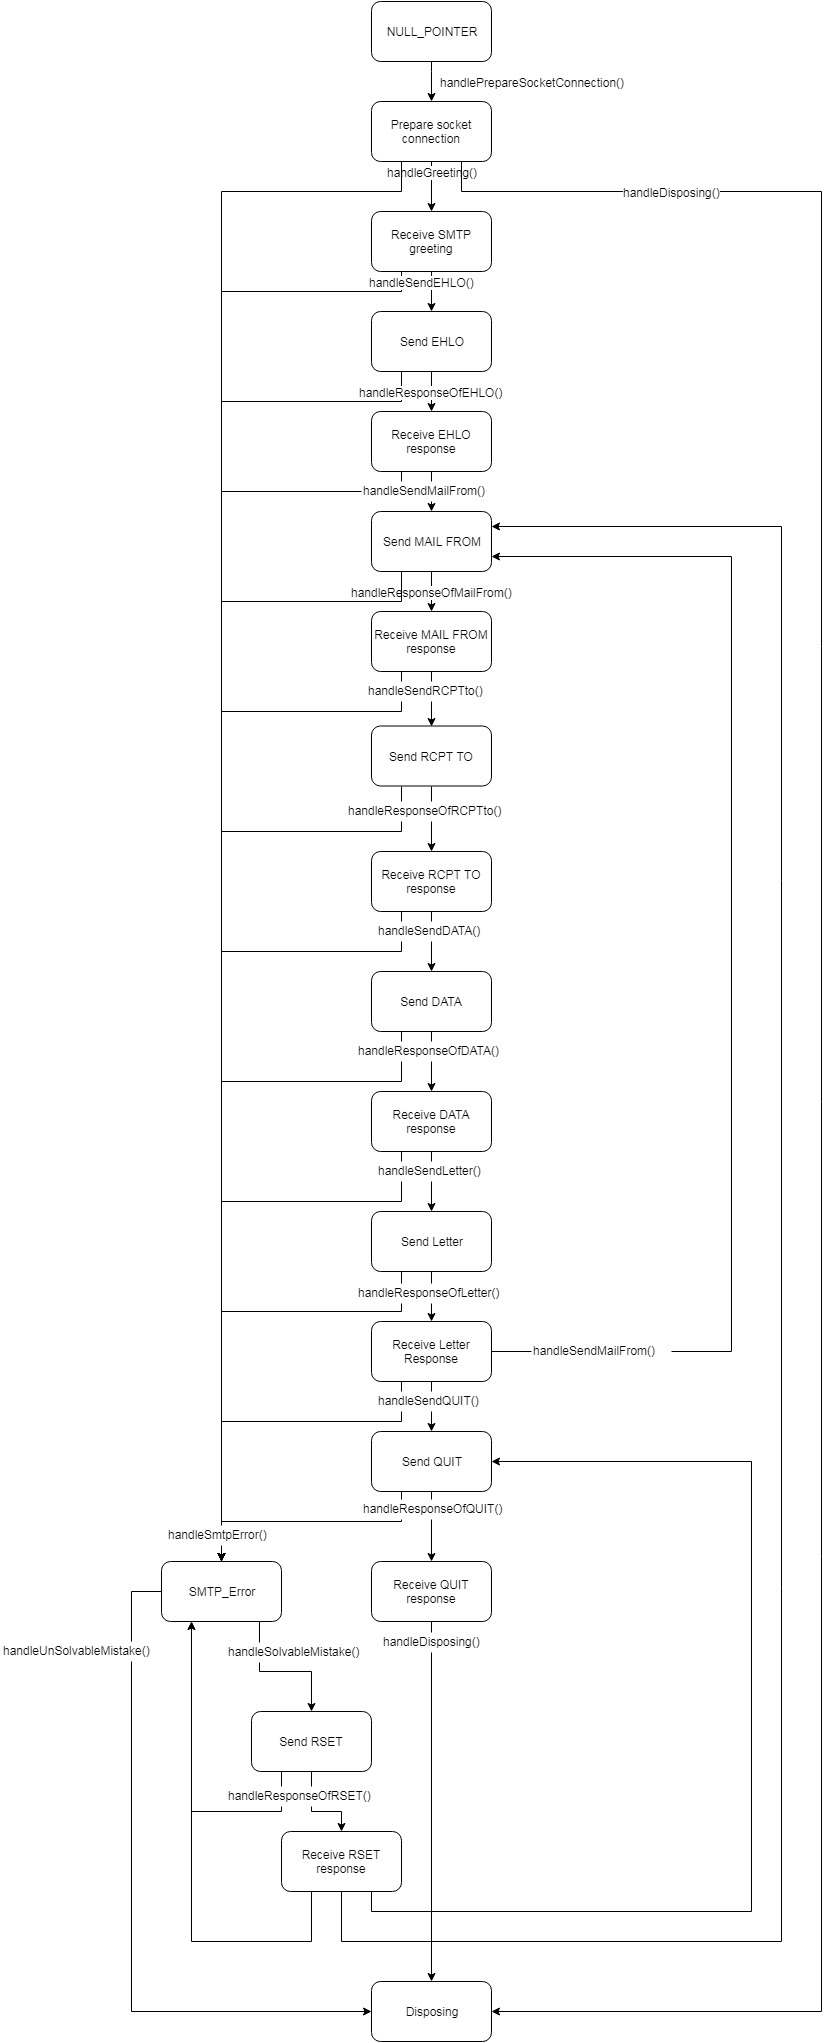
\includegraphics[height=\textheight]{static/ClientDiagram_Final.jpg}
\caption{Состояния сервера}
\label{fig:fsm}
\end{figure}

\section*{Клиент}

\subsection{Принцип действия}
Работу клиента можно разделить на 2 отдельные сущности: работа основного потока, работа рабочих потоков \textit{(далее воркеры)}
В основном потоке решено производить следующие действия
\begin{enumerate}
    \item Создание при инициализации и удаление при завершении списка воркеров
    \item Циклический поиск новых писем
    \item Распределение писем по воркерам
    \item Перехват сигналов на завершение работы
\end{enumerate}

При запуске сервера, главный поток создает пул воркереров и помещает в него логгер и рабочие потоки. Количество рабочих потоков напрямую зависит от количества процессоров на устройстве. Однако, для устройств в которых процессоров меньше чем 3 создается обязательно 1 рабочих процесс
Для \textit{Изящного завершения} необходимо подписаться на перехват сигналов. Для более корректного и однозначного управления потоками программы необходимо, чтобы рабочие потоки не перехватывали общие сигналы с главным потоком. Для этого решено использовать 2 сигнала \textbf{SIGINT} для завершения программы ~-- перехватывается главным потоком и \textbf{SIGUSR1} для управления воркерами. Во время корректного завершения главный поток оповещает всех воркеров по очереди в своем спике с помощью сигнала и ожидает их завершения. После завершения необходимо удалить данные воркера и освободить все ресурсы занимаемые главным потоком.

Рабочие процессы в данном случае выполняют роль связных. Их деятельность можно описать следующими действиями:
\begin{enumerate}
    \item Контролирует список соединений
    \item Получает и обрабатывает задания от главного потока
    \item Отправляет письма
\end{enumerate}

Воркер во время инициализации получает служебную информацию для поддержания связи с главным потоком. Так как в требованиях к заданию указывается, что соединение должно быть неблокируемым, каждый воркер обладает множествами пишущих, читающих и обработчиков прерываний. Помимо указаных множеств в данном блоке информации хранится список активных соединений (сокетов)
Во время работы воркер ожидает на \textbf{pselect} готовых к работе соединений. Однако, перед этим необходимо распределить новые задания от главного потока. После обработки всех заданий воркер для каждого готового соединения передает управление SMTP контроллеру до тех пор, пока:
\begin{itemize}
    \item Текущее состояние соединения - в процессе
    \item Текущее состояние соединения - заблокирован
    \item Дальнейших действий в SMTP контроллере по данному соединению произвести невозможно.
\end{itemize} 
Если по текущемо соединению все задания на текущий момент были завершены, то активное соединение удаляется из списка. 
Стоит отметить что, для того чтобы новые заявки не накапливались во время ожидания активных соединений, решено использовать таймер. Таким образом, все новые заявки будут распределяться по своим соединениям даже когда они не готовы.
Ранее, отмечалось, что воркер управляется главным потоком через сигнал. Он используется как для оповещения новых заданий, так и для завершения работы. Принцип \textit{"Изящного завершения"} должен учитывать состояния соединений воркера. Поэтому заверешние воркера заключается в уменьшении текущих задач. Для всех соединений задания, которые необходимо будет выполнить(не текущее) удаляется из списка заданий, а само письмо переноситься в начальную директорию (/new) пользователя. В случае, если соединение еще не было корректно установлено (для данного соединения еще не было приветствия от SMTP сервера), тогда первое задание тоже удаляется, файл переноситься, а соединение закрывается и удаляется. Текущие же задания, если стадия "приветствия" прошла успешно обрабатываются до конца. После обработки всех оставшихся соединений, воркер освобождает занимаемые им ресурсы и сообщает о завершении работы.

\subsection{Обработка новых писем}
Для отправки писем, необходимо найти письма в maildir и отправить их воркерам на выполнение. Функцию поиска писем выполняет главный поток. После инициализации всех необходимых структур и данных главный поток проверяет maildir на наличие новых писем. Сначала формируется список пользователей SMTP клиента. После, в каждой директории из списка проверяется директория \textbf{new} на наличие новых писем. Если в данном каталоге есть файлы, необходимо выделить информацию о адресате письма. Адресат письма получается из поля \textbf{To} письма. На его основе формируется домен, ответственный за прием писем пользователей. 
Найденное письмо перемещается в директорию \textbf{tmp} и для него формируется заявка на отправку. В заявке указан ответственный домен и путь к письму. После производится поиск подходящего воркера и задание на оптравку делегируется. Когда список файлов на отправку освобождается главный поток ожидает 30 секунд и повторяет поиск заново. Для корректного распределения используется метрика загруженности воркеров. Она отображает сколько задач уже было делегировано воркеру.

\subsection{Словарь}
Для контроля распределения заявок между воркерами, а так же отправки писем через одну соединение, хоть это и не обязательно, решено использовать словарь. В данном словаре хранится информация о распределении доменов между воркерами. Во время поиска писем, главный поток узнает ответственный домен и смотрит свой словарь доменов. Если в нем нет воркера, который уже работает с данным доменом, то выбирается наимение загруженный воркер. В случае если есть воркер, то новое письмо делегируется ему.
Рабочий процесс также взаимодействует с данным словарем. Когда список заданий для какого-либо определенного домена закончился, соединение переходит в режим "завершения" отправки писем. В данный момент и воркер удаляет запись в словаре для данного домена. Таким образом, система старается(не гарантирует) отправить все письма адресованные одному домену через одно активное соединение.

\subsection{Рабочий поток}
Каждый рабочий поток обладает записью с необходимой информацией о себе. Данная информация передается ему при создании. С помощью общей с главным потоком блоком информации, воркер может получать новые задания узнавать о текущем состоянии работы программы. В данном блоке целесообразно хранить следующую информацию:
\begin{itemize}
    \item ссылку на очередь новых заданий
    \item личный идентификатор (удобно для логгирования)
    \item состояние работы
    \item количество заданий
\end{itemize}
Доступ к очереди заданий рабочего процесса имею два потока: главный и сам рабочий поток. Для исключения коллизий, потери данных необходимо использовать объект синхронизации. В качестве такого объекта синхронизации является семафор. 
Для корректной работы, каждый воркер создает во время подготовки структуру, с помощью которой будет осуществляться контроль соединений и их состояний. Разграничение между состояниями соединений необходимо учитывать во время передачи данных. Для этого в данной структуре содержатся множества ожидающих на запись и ожидающих на чтение соединений. 

Параметр состояния работы, указывает рабочему процессу на необходимость корректного и быстрого завершения работы. В связи с этим, рабочий процесс, узнав о необходимости завершения, убирает все задания, которые еще не выполнялись у каждого соединения. Также изменяется время ожидания активизации соединений. Это необходимость обусловлена неблокируемостью сокетов, из-за чего у соединения нет как такого \textit{timeout} на получение или отправку. Стоит отметить, что у каждого соединения текущее задание остается для корректного завершения обмена информацией с серверами.

Каждое активное соединение обрабатывается с помощью SMTP контроллера

\subsection{Активное соедиение}
Каждое соедиенние должно быть однозначно определено. Для контроля соединений целесообразно описать соединение следующим образом
\begin{itemize}
    \item идентификатор соединения
    \item домен сервера
    \item адрес сервера
    \item текущее состояние соединения
    \item предыдущее состояние соединения
    \item количество попыток отправки одного письма
    \item список писем
    \item данные текущего письма
\end{itemize}

Во время подготовки к соединению необходимо разрешить адрес сервера. Для этого для указанного домена необходимо запросить MX запись. Из этой записи получается доменное имя самого SMTP сервера, с которым необходимо обмениваться данными. Однако, для корректного обмена необходимо узнать его IP адрес в сети. Для этого полученной записи запрашивается список IP адресов и выбирается первый успешно обработанный. 
Для оптимальной обработки писем, целесообразно хранить в памяти только служебную информацию, которая необходима для передачи письма. Для этих целей выделена отдельный блок "данные письма". В данной блоке хранится адресат и адресант письма. Это позволяет сократить время на открытия файл и взаимодействия с ним во время установленного соединения

\subsection{SMTP контроллер}
SMTP контроллер отвечает за корректность общения с серверами. Для контроля обмена информацией данный контроллер ослеживает состояния общения и ведет их учет. Таким образом исключается возможность непредвиденных переходов, отправки некорректного сообщения, а так же исключается очередность отправки/получения сообщений между SMTP клиентом и SMTP сервером. Состояния соединений и переходы между ними отображены на Рис. ~\ref{fig:smtp-client-states}

\begin{figure}
    \centering
    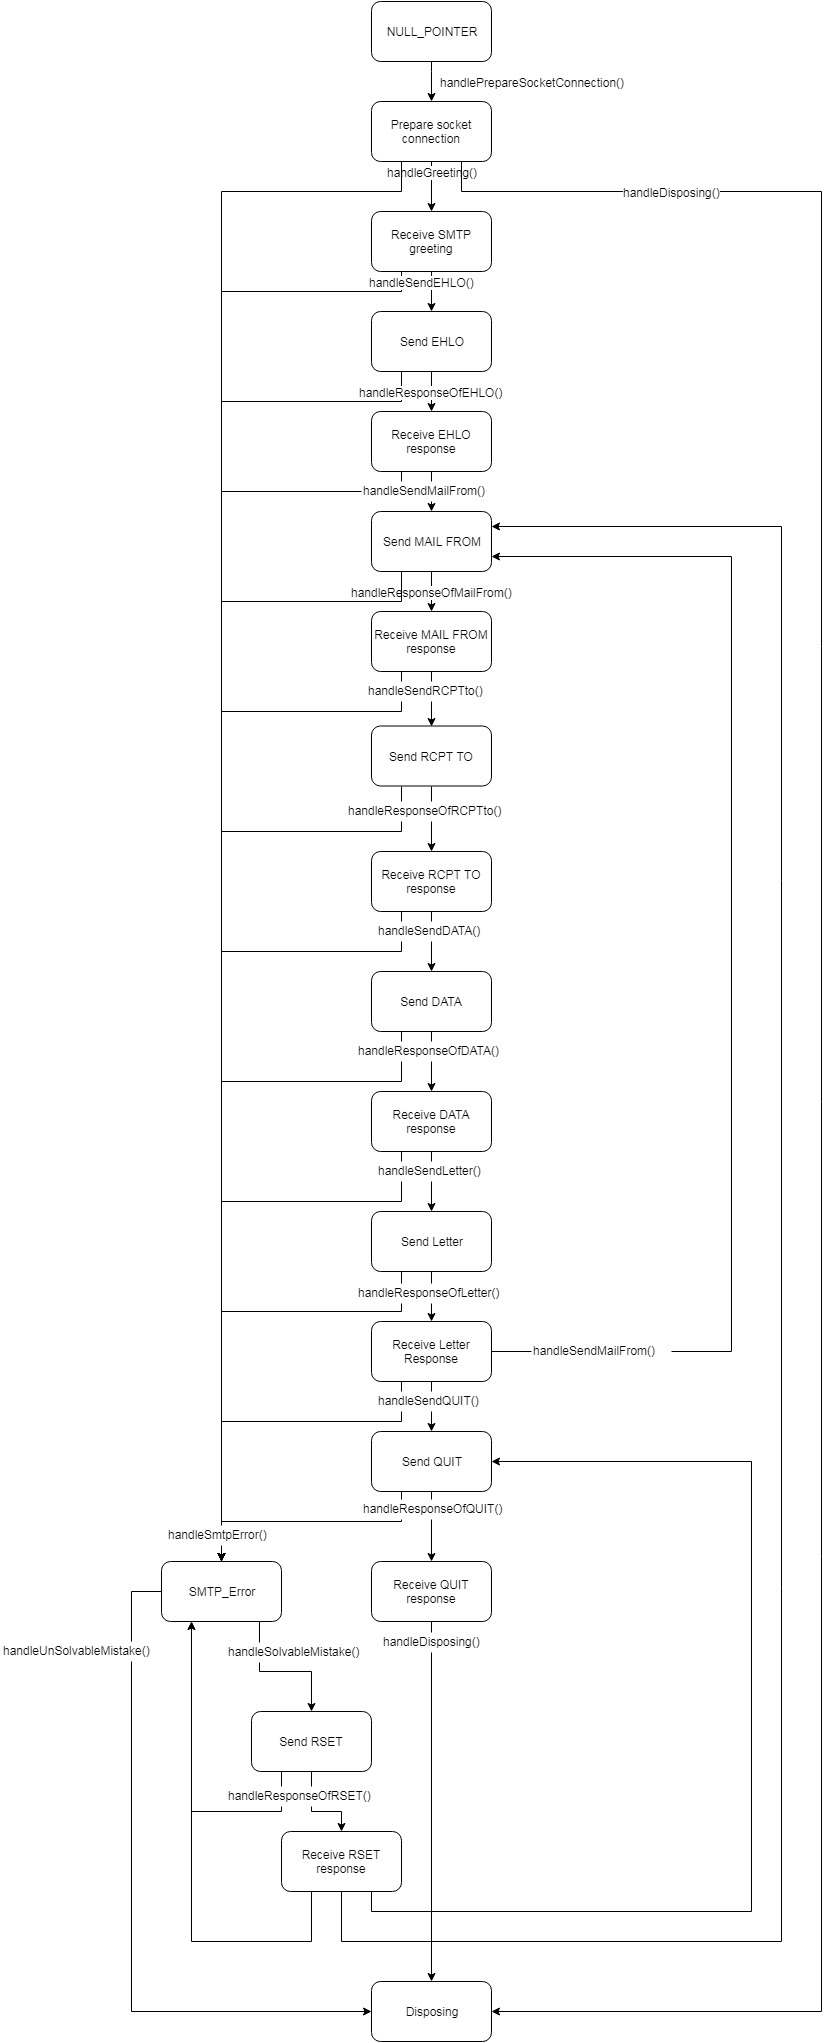
\includegraphics[height=\textheight]{static/ClientDiagram_Final.jpg}
    \caption{Конечный автомат cостояний соединений SMTP клиента}
    \label{fig:smtp-client-states}
\end{figure}

Стоит отметить, что во при переходе к завершению обмена данными по данному соединение именно SMTP контроллер удаляет запись из \textit{словаря}. Это необходимо для исключения появления писем по закрывающемуся соединению. Таким образом, главный поток не будет делегировать письма воркеру, который завершает процесс передачи для данного домена и выберет наиболее свободного воркера.
Отправка команд протокола SMTP сопровождается верификацией ответов от сервера. Каждый ответ сервера проверяется на соблюдение регламента передачи. Так, во время подключения к SMTP серверу и получения сообщения от сервера с доменным именем за который он отвечает, происходит верификация статуса ответа и самого домена. В случае нарушения соглашения: некорректный ответ или указанный в сообщение домен не совпадает с указанным в соединение, возникает ошибка, которая разрешается закрытием соединения и освобождению ресурсов.

\subsection{Синтаксис поддерживаемых команд протокола}
В данном разделе приведены поддерживаемые клиентом команды протокола SMTP.

\begin{itemize}
    \item \textbf{EHLO}: {\it EHLO [w+]+\/}
    \item \textbf{MAIL}: {\it MAIL FROM: <[\textbackslash w]+@[\textbackslash w]+\.[\textbackslash w]+>\/}
    \item \textbf{RCPT}: {\it RCPT To:<[\textbackslash w]+@[\textbackslash w]+\.[\textbackslash w]+>\/}
    \item \textbf{DATA}: {\it DATA\/}
    \item \textbf{RSET}: {\it RSET\/}
    \item \textbf{QUIT}: {\it QUIT\/}
\end{itemize}

% \begin{itemize}
%     \item EHLO <my_domain><CRLF>
%     \item MAIL FROM:< <sender> > <CRLF>
%     \item RCPT To:< <destination> > <CRLF>
%     \item DATA <CRLF> 
%     \item QUIT <CRLF>
%     \item RSET <CRLF>
% \end{itemize}

\chapter{Технологический раздел}

\section{Сборка программы}

Сборка программы, как для сервера, так и для клиента, осуществляется с помощью Makefile, объединяющего в себе несколько целей:
\begin{enumerate}
\item сборка исполняемого файла сервера/клиента (по умолчанию),
\item сборка модульных тестов,
\item генерация автомата состояний.
\end{enumerate}
Генерация отчета по данному проекту осуществляется в единственном экземпляре и файл отчета содержит в себе данные как для сервера, так и для клиента. Для этой цели был создан отдельный Makefile с целями для генерации непосредственно отчета, а также включаемых данных, таких как, например, графы вызовов функций.

\section{Сервер}

\section{Графы вызова функций}

Поскольку функций много, графы вызовов разбиты на два рисунка. На рис.~\ref{fig:ccflow01} показаны основные функции, на рис.~\ref{fig:scflow01}~-- функции обработки команд. Файл \textbf{cflow.ignore} содержит список функций (точнее, шабловнов поиска), использыемых программой \textit{grep} для удаления малоинтересных стандартных функций\footnote{Функции по работе с сокетами, ipc и привилегиями к малоинтересным ни в коем случае не относятся.}.


\begin{figure}
\centering
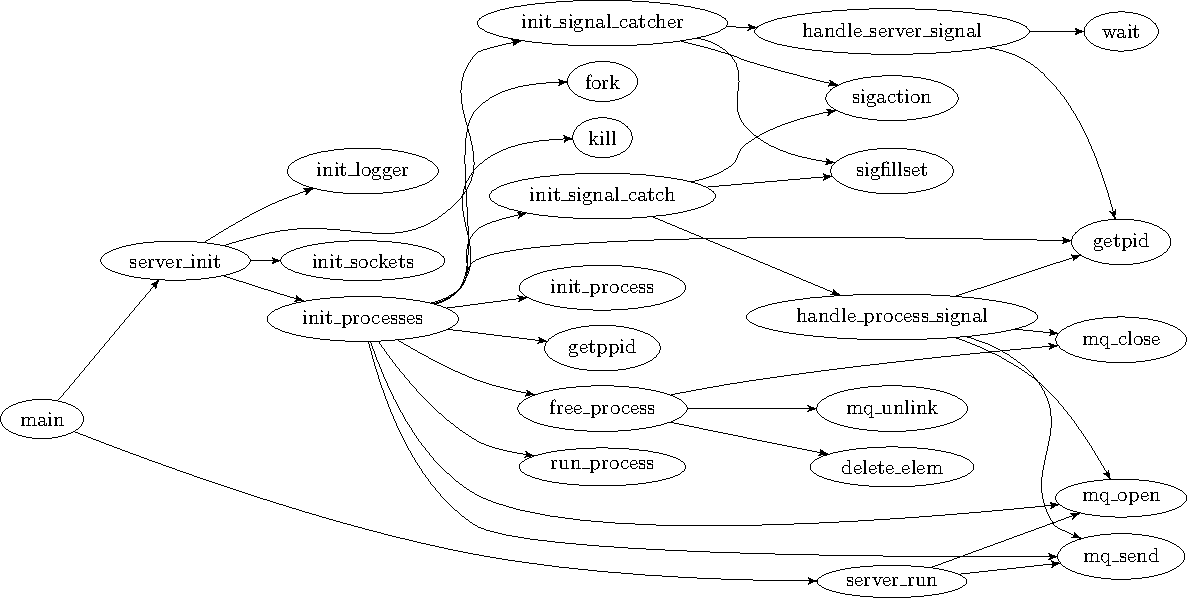
\includegraphics[width=\textwidth]{include/scflow01_dot.pdf}
\caption{Граф вызовов, функции обработки команд}
\label{fig:scflow01}
\end{figure}

\begin{figure}
\centering
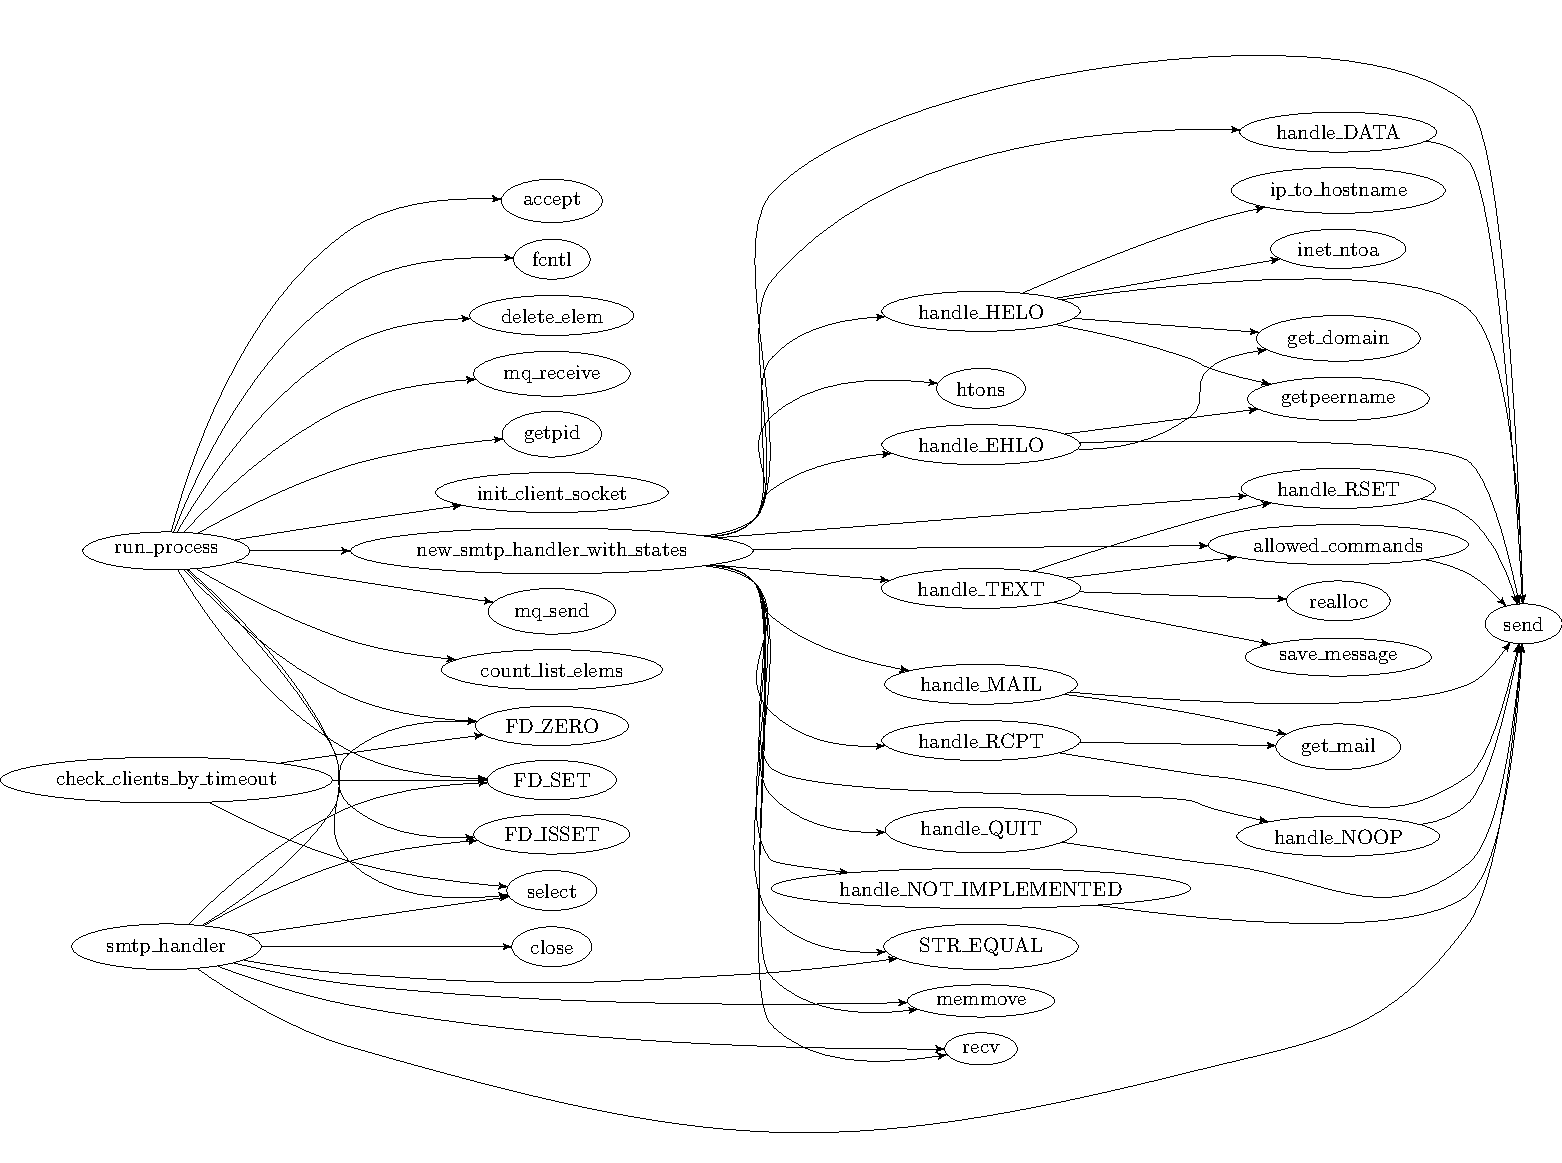
\includegraphics[width=\textwidth]{include/scflow02_dot.pdf}
\caption{Граф вызовов, функции обработки команд}
\label{fig:scflow01}
\end{figure}

Графы созданы с помощью \textit{cflow}, \textit{cflow2dot}, \textit{dot}.


\section{Клиент}

\subsection{Графы вызова функций}

\begin{figure}
    \centering
    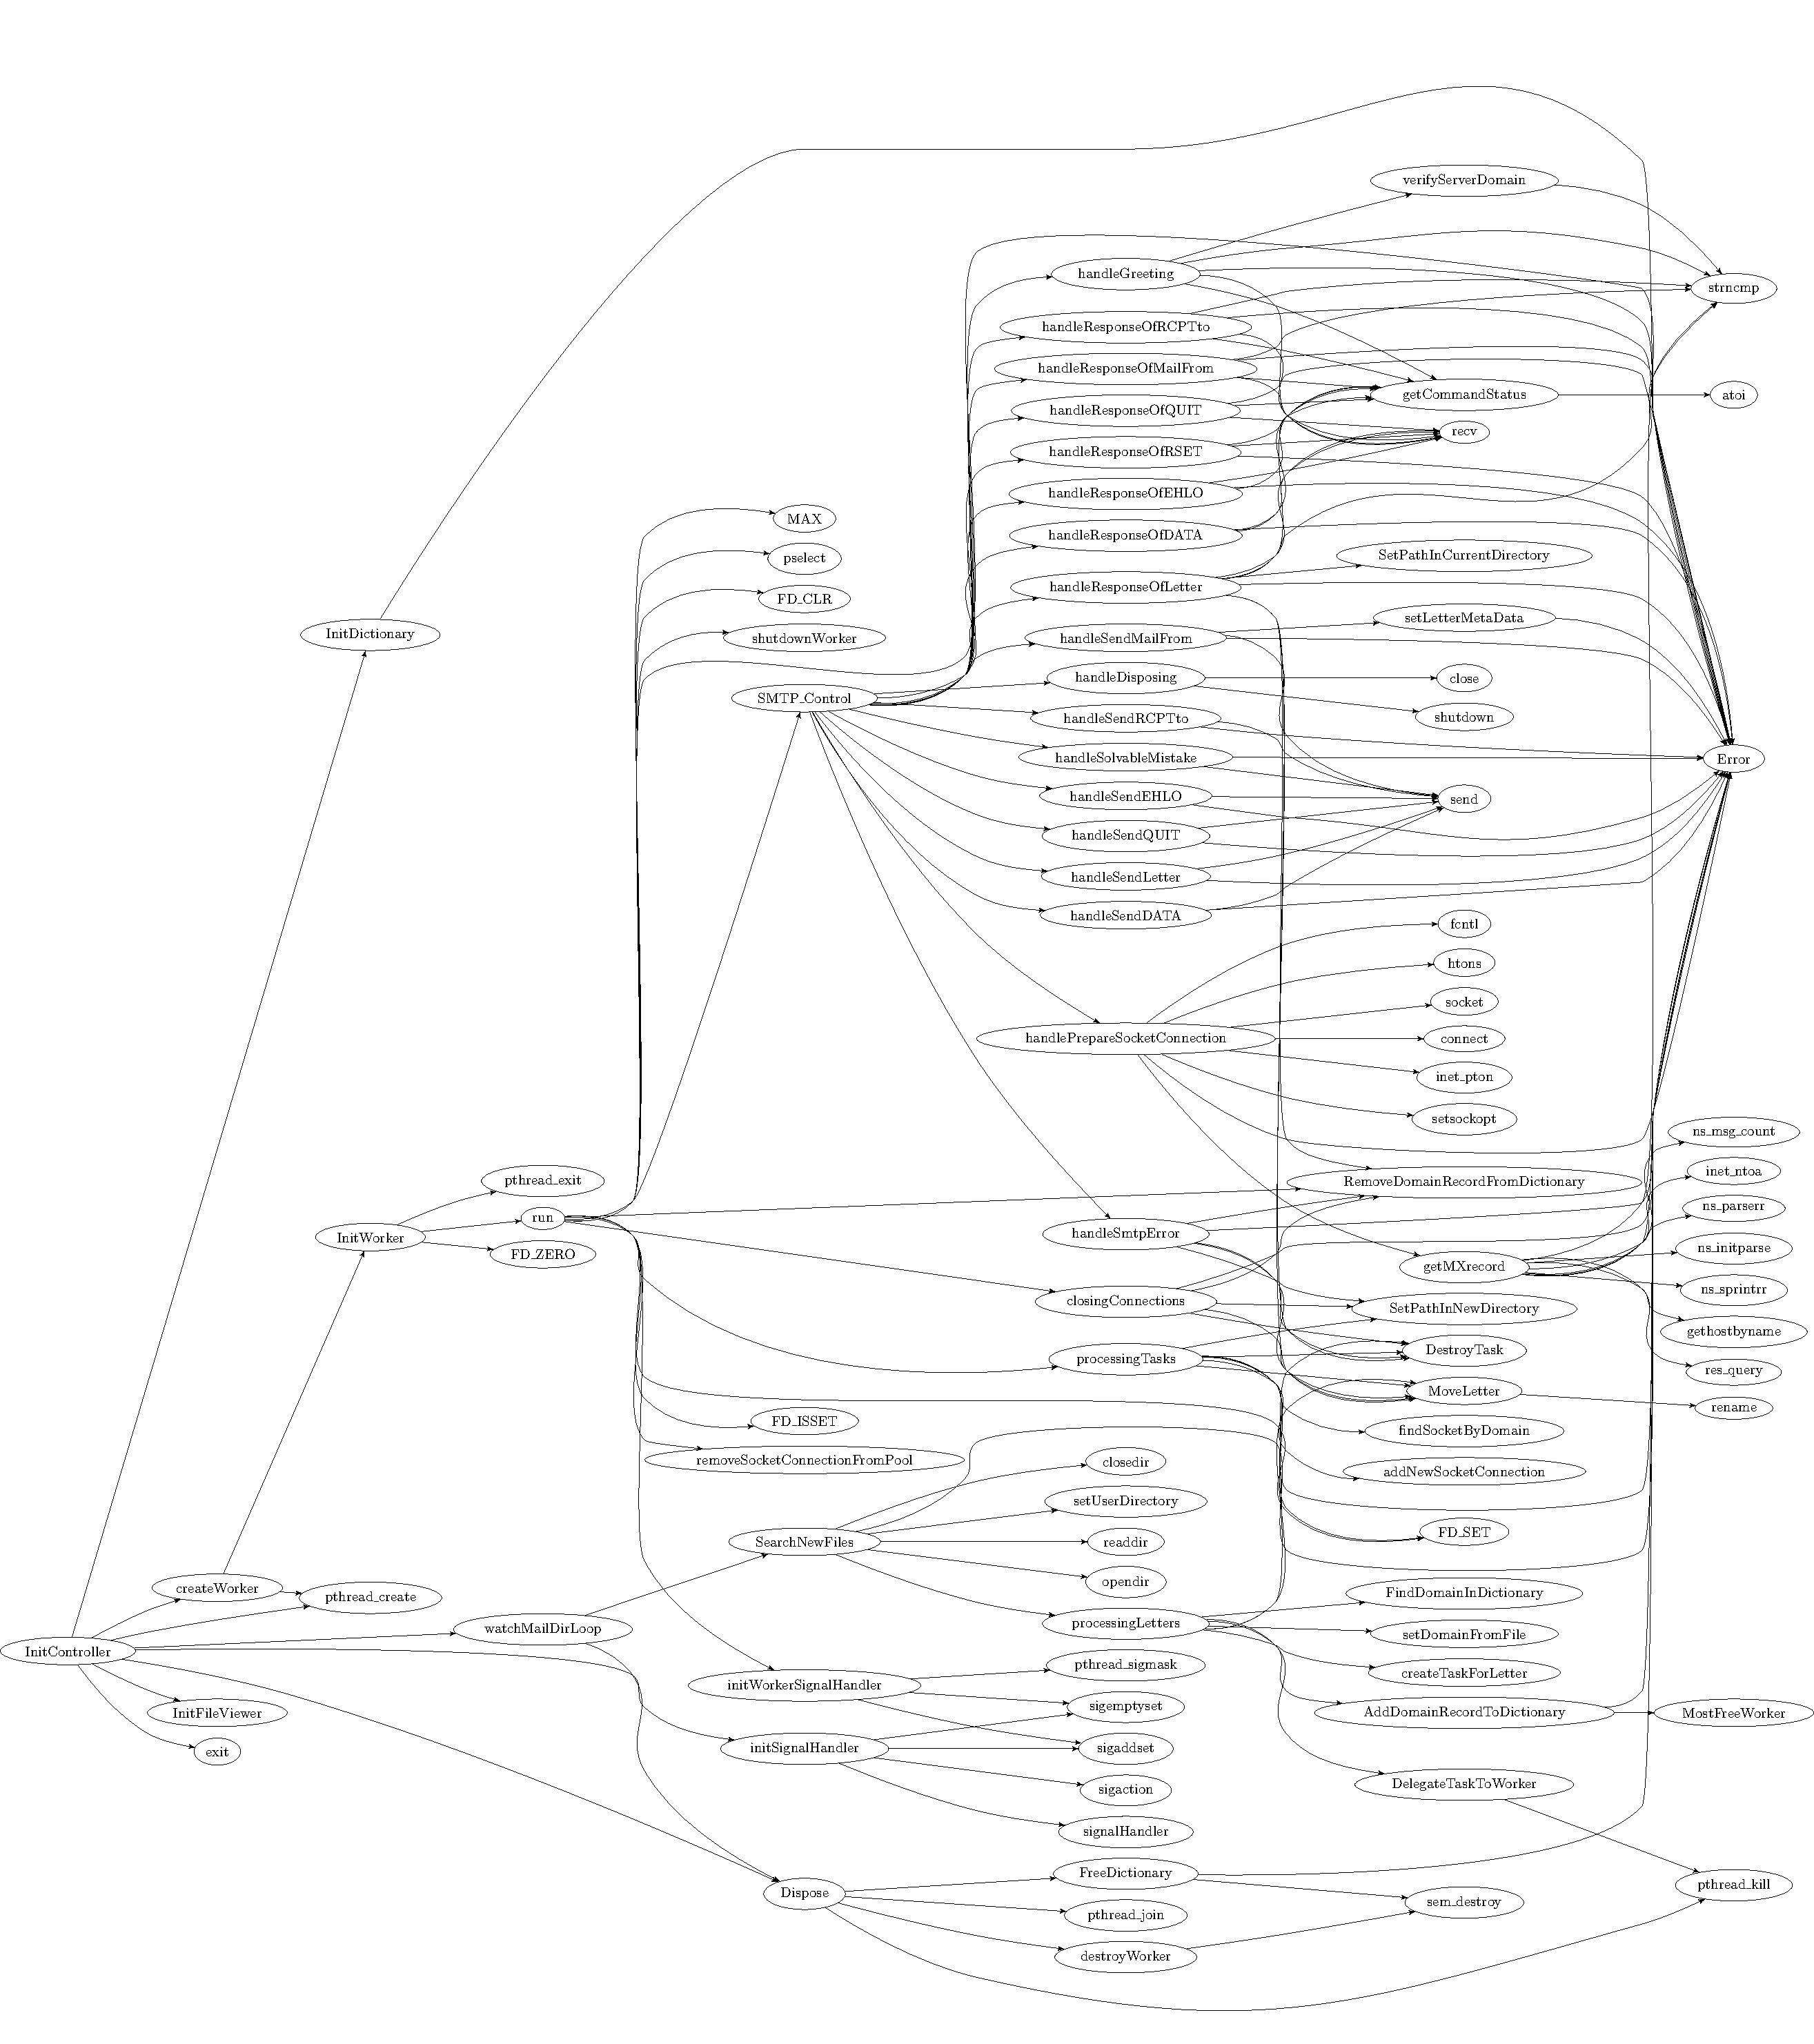
\includegraphics[width=\textwidth]{include/ccflow01_dot.pdf}
    \caption{Граф вызовов, основные функции}
    \label{fig:ccflow01}
\end{figure}
    
\begin{figure}
    \centering
    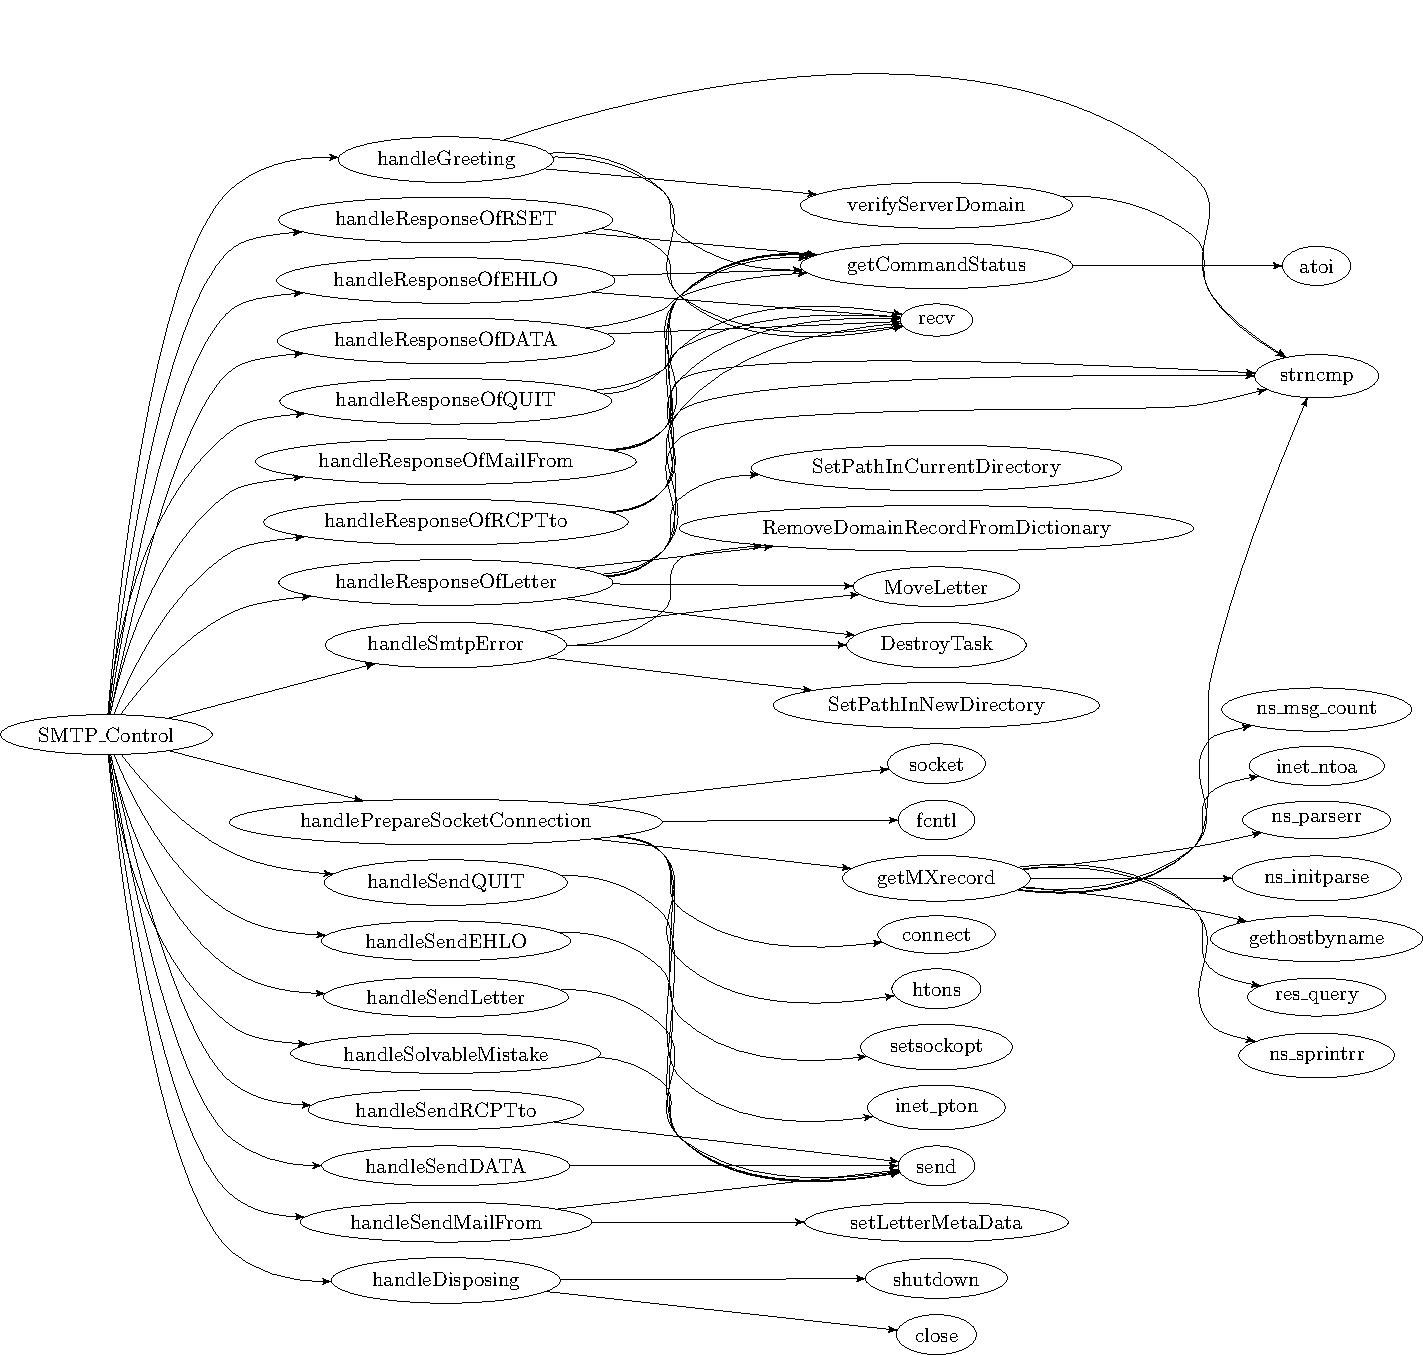
\includegraphics[width=\textwidth]{include/ccflow02_dot.pdf}
    \caption{Граф вызовов, взаимодействие с сервером}
    \label{fig:ccflow02}
\end{figure}

\subsection{Основные данные}

Стркутура рабочего процесса
\begin{verbatim}
    struct worker
    {
        pthread_t thread;
        sem_t lock;
        struct worker_task *tasks;
        int workerId;
        int count_task;
        bool worked;
    };
\end{verbatim}

Структура соединения
\begin{verbatim}
    struct FileDesc
    {
        int id;
        char *domain;
        char *mx_record;
        struct sockaddr_in addr;
        int current_state;
        int prev_state;
        int attempt;
        struct worker_task *task_pool;
        struct letter_info meta_data;
    };
\end{verbatim} 

\subsection{Тестирование}

\subsection{Сервер}
Модульные тесты создаются с помощью сценария unit\_tests. Ниже приведён отчет о модульном тестировании (с использованием библиотеки CUnit):
\subsection{Сервер - модульные тесты}
\begin{verbatim}
     CUnit - A unit testing framework for C - Version 2.1-2 \\
     http://cunit.sourceforge.net/ \\


Suite: suite_test \\
  Test: create_client_socket_no_message ...passed \\
  Test: create_client_socket_has_message ...passed \\
  Test: handle_helo_state_init ...Server: 0, HELO: 252 Ok \\
 myserver.com \\
passed \\
  Test: handle_helo_state_incorrect ...passed \\
  Test: handle_ehlo_state_correct ...Server: 0, EHLO: 250- myserver.com \\
passed \\
  Test: handle_ehlo_state_incorrect ...passed \\
  Test: handle_mail_correct ...Server: 0, MAIL: test@test.ru 250 Ok \\
passed \\
  Test: handle_mail_incorrect_command ...Server: 0, MAIL: 450 Requested mail action not taken: mailbox unavailable \\
passed \\
  Test: handle_mail_incorrect_state ...passed \\
  Test: handle_rcpt_correct ...Server: 0, RCPT: 250 Ok \\
passed \\
  Test: handle_rcpt_incorrect_command ...Server: 0, MAIL: 450 Requested mail action not taken: mailbox unavailable \\
passed \\
  Test: handle_rcpt_incorrect_state ...passed \\
  Test: handle_rcpt_exceeded_recepients ...Server: 0, RCPT: 250 Ok \\
Server: 0, RCPT: 250 Ok \\
Server: 0, RCPT: 250 Ok \\
Server: 0, RCPT: 250 Ok \\
Server: 0, RCPT: 250 Ok \\
Server: 0, RCPT: 250 Ok \\
Server: 0, RCPT: 250 Ok \\
Server: 0, RCPT: 250 Ok \\
Server: 0, RCPT: 250 Ok \\
Server: 0, RCPT: 250 Ok \\
Server: 0, RCPT: 451 Unable to complete command: number of recipients exceeded \\
passed \\
  Test: handle_rset_correct_no_recepients ...Server: 0, RSET: 250 Ok reset \\
passed \\
  Test: handle_rset_correct_has_recepients ...Server: 0, RSET: 250 Ok reset \\
passed \\
  Test: handle_rset_incorrect_state ...passed \\
  Test: test_prepare_client_before_getting_data_no_reset ...Server: 0, HELO: 252 Ok \\
 myserver.com \\
Server: 0, MAIL: test@test.ru 250 Ok \\
Server: 0, RCPT: 250 Ok \\
passed \\
  Test: handle_data_correct ...Server: 0, DATA: 354 Start mail input; end with <CRLF>.<CRLF> \\
passed \\
  Test: handle_data_incorrect_state ...passed \\
  Test: handle_quit_correct ...Server: 0, QUIT: 221 Ok \\
passed \\
  Test: handle_noop_correct ...Server: 0, NOOP: 250 Ok noop \\
passed \\
  Test: handle_not_implemented_correct ...Server: 0, NOT_IMPLEMENTED: 502 Command Not Implemented \\
passed \\
  Test: handle_text_not_dot ...Client: 0, In-MESSAGE: Test messsage passed \\
  Test: test_full_session_correct ...Server: 0, HELO: 252 Ok \\
 myserver.com \\
Server: 0, MAIL: test@test.ru 250 Ok \\
Server: 0, RCPT: 250 Ok \\
Server: 0, DATA: 354 Start mail input; end with <CRLF>.<CRLF> \\
Client: 0, In-MESSAGE: .Server: 0, MESSAGE: Server: 0, RSET: 250 Ok reset \\
Server: 0, QUIT: 221 Ok \\
passed \\
 \\
Run Summary:   \_ Type  \_Total \_   Ran Passed\_ Failed\_ Inactive \\
          \_    suites  \_    1   \_   1   \_ n/a    \_  0    \_    0 \\
          \_     tests  \_   24  \_   24    \_24     \_ 0    \_    0 \\
          \_   asserts  \_  126  \_  126  \_  126   \_   0  \_    n/a \\

Elapsed time =    0.003 seconds \\

\end{verbatim}
\subsection{Сервер - valgrind}
Ниже приведен пример вывода для утилиты валгринд (число процессов = 2) \\

\begin{verbatim}
==6831== HEAP SUMMARY: \\
==6831==     in use at exit: 644 bytes in 4 blocks \\
==6831==   total heap usage: 106 allocs, 102 frees, 28,505 bytes allocated \\
==6831==  \\
==6831== Searching for pointers to 4 not-freed blocks \\
==6831== Checked 104,096 bytes \\
==6831==  \\
==6831== LEAK SUMMARY:\\
==6831==    definitely lost: 0 bytes in 0 blocks\\
==6831==    indirectly lost: 0 bytes in 0 blocks\\
==6831==      possibly lost: 0 bytes in 0 blocks\\
==6831==    still reachable: 644 bytes in 4 blocks\\
==6831==         suppressed: 0 bytes in 0 blocks\\
==6831== Reachable blocks (those to which a pointer was found) are not shown.\\
==6831== To see them, rerun with: --leak-check=full --show-leak-kinds=all\\
==6831== \\
==6831== ERROR SUMMARY: 0 errors from 0 contexts (suppressed: 0 from 0)\\
==6831== ERROR SUMMARY: 0 errors from 0 contexts (suppressed: 0 from 0)\\
\\
\\
==6830== HEAP SUMMARY:\\
==6830==     in use at exit: 40 bytes in 3 blocks\\
==6830==   total heap usage: 8 allocs, 5 frees, 1,060 bytes allocated\\
==6830== \\
==6830== Searching for pointers to 3 not-freed blocks\\
==6830== Checked 103,504 bytes\\
==6830== \\
==6830== LEAK SUMMARY:\\
==6830==    definitely lost: 0 bytes in 0 blocks\\
==6830==    indirectly lost: 0 bytes in 0 blocks\\
==6830==      possibly lost: 0 bytes in 0 blocks\\
==6830==    still reachable: 40 bytes in 3 blocks\\
==6830==         suppressed: 0 bytes in 0 blocks\\
==6830== Reachable blocks (those to which a pointer was found) are not shown.\\
==6830== To see them, rerun with: --leak-check=full --show-leak-kinds=all\\
==6830== \\
==6830== ERROR SUMMARY: 3 errors from 2 contexts (suppressed: 0 from 0)\\
\\
==6833== HEAP SUMMARY:\\
==6833==     in use at exit: 92 bytes in 5 blocks\\
==6833==   total heap usage: 12 allocs, 9 frees, 1,768 bytes allocated\\
==6833== \\
==6833== Searching for pointers to 5 not-freed blocks\\
==6833== Checked 103,592 bytes\\
==6833== LEAK SUMMARY:\\
==6833==    definitely lost: 52 bytes in 2 blocks\\
==6833==    indirectly lost: 0 bytes in 0 blocks\\
==6833==      possibly lost: 8 bytes in 1 blocks\\
==6833==    still reachable: 32 bytes in 2 blocks\\
==6833==         suppressed: 0 bytes in 0 blocks\\
==6833== Reachable blocks (those to which a pointer was found) are not shown.\\
==6833== To see them, rerun with: --leak-check=full --show-leak-kinds=all\\
==6833== \\
==6833== Use --track-origins=yes to see where uninitialised values come from\\
==6833== ERROR SUMMARY: 10 errors from 10 contexts (suppressed: 0 from 0)\\
\\
==6832== HEAP SUMMARY:\\
==6832==     in use at exit: 185 bytes in 7 blocks\\
==6832==   total heap usage: 33 allocs, 29 frees, 10,976 bytes allocated\\
==6832== \\
==6832== Searching for pointers to 8 not-freed blocks\\
==6832== Checked 103,592 bytes\\
\\
==6832== \\
==6832== LEAK SUMMARY:\\
==6832==    definitely lost: 132 bytes in 3 blocks\\
==6832==    indirectly lost: 13 bytes in 1 blocks\\
==6832==      possibly lost: 0 bytes in 0 blocks\\
==6832==    still reachable: 40 bytes in 3 blocks\\
==6832==         suppressed: 0 bytes in 0 blocks\\
==6832== Reachable blocks (those to which a pointer was found) are not shown.\\
==6832== To see them, rerun with: --leak-check=full --show-leak-kinds=all\\
==6832== \\
==6832== Use --track-origins=yes to see where uninitialised values come from\\
==6832== ERROR SUMMARY: 12 errors from 12 contexts (suppressed: 0 from 0)\\
==6832== \\
\end{verbatim}

\begin{verbatim}
    CUnit - A unit testing framework for C - Version 2.1-3
     http://cunit.sourceforge.net/


    Suite: suite_test
    Test: domain_is_NULL ...passed
    Test: bad_domain ...passed
    Test: connection_is_blocked ...passed
    Test: greeting_bad_graph_state ...passed
    Test: in_greeting_not_correct_domain ...passed
    Test: send_ehlo_and_correct_result ...passed
    Test: send_ehlo_and_change_state_on_error ...passed

    Run Summary:    Type  Total    Ran Passed Failed Inactive
                suites      1      1    n/a      0        0
                tests      7      7      7      0        0
                asserts     24     24     24      0      n/a

    Elapsed time =    0.004 seconds
\end{verbatim}

\subsection{Valgrind}

\begin{verbatim}
    ==24216== LEAK SUMMARY:
    ==24216==    definitely lost: 326 bytes in 6 blocks
    ==24216==    indirectly lost: 1,056 bytes in 4 blocks
    ==24216==      possibly lost: 272 bytes in 1 blocks
    ==24216==    still reachable: 1,638 bytes in 4 blocks
    ==24216==         suppressed: 0 bytes in 0 blocks
    ==24216== Reachable blocks (those to which a pointer was found) are not shown.
    ==24216== To see them, rerun with: --leak-check=full --show-leak-kinds=all
    ==24216== 
    ==24216== For counts of detected and suppressed errors, rerun with: -v
    ==24216== Use --track-origins=yes to see where uninitialised values come from
    ==24216== ERROR SUMMARY: 33 errors from 21 contexts (suppressed: 0 from 0)
\end{verbatim}

\subsection{Пример работы относительно сервер}

\begin{verbatim}
    11 Jan 2019 00:07:51 DEBUG org.subethamail.smtp.server.Session - Server: 220 samsung-np530u4c ESMTP SubEthaSMTP null
    11 Jan 2019 00:07:51 DEBUG org.subethamail.smtp.server.Session - Client: EHLO samsung-np530u4c
    11 Jan 2019 00:07:51 DEBUG org.subethamail.smtp.server.Session - Server: 250-samsung-np530u4c
    250-8BITMIME
    250-AUTH LOGIN
    250 Ok
    11 Jan 2019 00:07:58 DEBUG org.subethamail.smtp.server.Session - Client: MAIL FROM:<mail.ru>
    11 Jan 2019 00:07:58 DEBUG org.subethamail.smtp.server.Session - Server: 250 Ok
    11 Jan 2019 00:07:58 DEBUG org.subethamail.smtp.server.Session - Client: RCPT To: <samsung-np530u4c>
    11 Jan 2019 00:07:58 DEBUG org.subethamail.smtp.server.Session - Server: 250 Ok
    11 Jan 2019 00:08:01 DEBUG org.subethamail.smtp.server.Session - Client: DATA
    11 Jan 2019 00:08:01 DEBUG org.subethamail.smtp.server.Session - Server: 354 End data with <CR><LF>.<CR><LF>
    11 Jan 2019 00:08:02 DEBUG org.subethamail.smtp.server.Session - Server: 250 Ok
    11 Jan 2019 00:08:07 DEBUG org.subethamail.smtp.server.Session - Client: MAIL FROM:<mail.ru>
    11 Jan 2019 00:08:07 DEBUG org.subethamail.smtp.server.Session - Server: 250 Ok
    11 Jan 2019 00:08:07 DEBUG org.subethamail.smtp.server.Session - Client: RCPT To: <samsung-np530u4c>
    11 Jan 2019 00:08:07 DEBUG org.subethamail.smtp.server.Session - Server: 250 Ok
    11 Jan 2019 00:08:08 DEBUG org.subethamail.smtp.server.Session - Client: DATA
    11 Jan 2019 00:08:08 DEBUG org.subethamail.smtp.server.Session - Server: 354 End data with <CR><LF>.<CR><LF>
    11 Jan 2019 00:08:10 DEBUG org.subethamail.smtp.server.Session - Server: 250 Ok
    11 Jan 2019 00:08:17 DEBUG org.subethamail.smtp.server.Session - Client: QUIT
    11 Jan 2019 00:08:17 DEBUG org.subethamail.smtp.server.Session - Server: 221 Bye
\end{verbatim}

% Нужно отметьть, что символ <<\_>> необходимо оформлять как <<\textbackslash\_>>.

\addcontentsline{toc}{chapter}{Выводы}
\chapter{Выводы}

В рамках предложенной работы нами были реализованы два компонента современного SMTP-сервера, взаимодействующих между самой по самописному протоколу в соответствии со стандартами RFC. В ходе работы реализованы следующие задачи: \\
\begin{enumerate}
	\item Сервер- Проанализировали архитектурное решение
    \item Сервер- Разработали подход для обработки входящих соединений и хранения входящих писем в maildir
    \item Сервер- Рассмотрели \textbf{SMTP}-протокол
    \item Сервер- Реализовали программу для получения писем по протоколу \textbf{SMTP}
    \item Клиент- Проанализировали архитектурное решение maildir
    \item Клиент- Разработали подход для обработки писем в maildir 
    \item Клиент- Рассмотрели \textbf{SMTP}-протокол
    \item Клиент- Проанализировали способы получения и обработки \textbf{MX}-записей
    \item Клиент- Реализовали программу для отправки писем по протоколу \textbf{SMTP}
    \item Общее- Рассмотрели работу с неблокирующими сокетами и их взаимодействие поверх протокола TCP
    \item Общее- Разработали системы, работающие в многозадачном режиме, столкнувшись с проблемами взаимодействия потоков и процессов, которые были решены в ходе работы
    \item Общее- Познакомились с утилитами автоматической сборки и тестирования
    \item Общее- Разработали сценарии тестирования для модулей протокола обработки сообщений, организовали определенный процент покрытия
    \item Общее- Познакомились с концепцией graceful shutdown, произвели ее реализацию в проекте.
\end{enumerate}


\end{document}
